%%%%%%%%%%%%%%%%%%%%%%%%%%%%%%%%%%%%%%%%%%%%%%%%%%%%%%%%%%%%%%%%%%%
%% introducao.tex
%% UNL thesis document file
%%%%%%%%%%%%%%%%%%%%%%%%%%%%%%%%%%%%%%%%%%%%%%%%%%%%%%%%%%%%%%%%%%%
\newcommand{\unlthesis}{\emph{unlthesis}}
\newcommand{\unlthesisclass}{\texttt{unlthesis.cls}}


\chapter{Introdução}
\label{cha:introdução}

%\begin{quotation}
%  \itshape
%  This work is licensed under the Creative Commons Attribution-NonCommercial~4.0 International License.
%  To view a copy of this license, visit \url{http://creativecommons.org/licenses/by-nc/4.0/}.
%\end{quotation}
\section{Uma curta apresentação} % (fold)
\label{sec:uma_curta_apresentação}

Ao longo dos anos, o número de defeitos e falhas nas estradas tem vindo a aumentar, mostrando-se um problema cada vez mais importante na vida de muitos cidadãos, especialmente os que fazem da condução a sua profissão. De modo a caminhar em direção à resolução deste problema, surgiu a oportunidade de realizar o projeto aqui apresentado, em que será sugerida uma das muitas soluções possíveis, utilizando uma abordagem que está diretamente ligada ao rápido aumento de utilizadores de telemóvel bem como ao grande número de condutores em Portugal, visto que existem cerca de 19 milhões de telemóveis em Portugal\footnote{http://www.pordata.pt/Portugal/Assinantes+++equipamentos+de+utilizadores+do+servi\%C3
\%A7o+m\%C3\%B3vel-1180} para os cerca de 11 milhões de habitantes na mesma região\footnote{http://www.pordata.pt/Portugal/Popula\%C3\%A7\%C3\%A3o+residente+total+e+por+grupo+et
\%C3\%A1rio-10}.

Surge então a necessidade de uma monitorização das vias de trânsito para a sua manutenção e reparação. Desta forma, tentando aliar a tecnologia com essa mesma necessidade, será desenvolvido um sistema que irá ser integrado em automóveis e que fará a deteção e comunicação de defeitos nas estradas com o telemóvel de cada automobilista.

Este documento irá fornecer, da forma mais detalhada possível, uma pequena introdução sobre quais os componentes necessários para construir um sistema de deteção de defeitos existentes nas estradas, utilizando um acelerómetro e um telemóvel, bem como comunicação \emph{Bluetooth} e \emph{wi-fi}, de modo a estabelecer a comunicação entre os vários componentes do sistema. Serão também apresentados os diversos pontos fortes e fracos da solução tomada, fazendo a comparação com projetos já desenvolvidos e as suas respetivas soluções.

\section{Montagem do sistema}
\label{sec:montagem_do_sistema}

O sistema que será desenvolvido terá como principal objetivo utilizar o máximo de componentes existentes num \emph{smartphone}, tornando-o o mais compacto e barato possível. Como tal, primeiro é necessário identificar quais os componentes essenciais para que seja possível o desenvolvimento do projeto, entre os quais se destacam o acelerómetro e o GPS, bem como módulos de comunicação \emph{Bluetooth} e \emph{wi-fi}/\emph{3G}.

\subsection{Componentes montados no veículo}
\label{subsec: componentes_montados_no_veiculo}

De modo a poder obter dados mais precisos, será considerada a utilização de um acelerómetro externo ao telemóvel, preso ao amortecedor do veículo para que seja possível obter diretamente as leituras quando um condutor passa num buraco da estrada, tornando assim a recolha de dados consistente uma vez que instalado, o acelerómetro não será mais movido. Os dados obtidos têm que ser registados e enviados para o telemóvel e para que tal seja possível, é necessária a existência de algum processador que faça esta gestão. De momento está a ser considerada a utilização de um \emph{arduino} ou um \emph{raspberry pi} para fazer o processamento dos dados e o posterior envio. Uma vez que os dados serão processados no telemóvel, esta decisão ainda não é definitiva pois poderá surgir uma opção economicamente mais viável. Para o envio dos dados será considerada a comunicação \emph{Bluetooth} uma vez que esta tecnologia se integra facilmente com vários processadores e está bastante desenvolvida, possibilitando uma escolha mais acertada.

\subsection{Componentes do telemóvel}
\label{subsec: componentes_do_telemovel}

Continuando com a montagem até agora descrita, torna-se claro que será utilizado o módulo \emph{Bluetooth}	do telemóvel para que este possa receber dados do acelerómetro. Quando for recebida a informação da deteção de um buraco, o GPS do telemóvel será ativado para que sejam obtidas as coordenadas em que este se encontra e para que posteriormente as informações possam ser cruzadas e armazenadas. O sistema de deteção fica completo com o envio de todos os dados obtidos para uma base de dados via \emph{wi-fi} ou \emph{3G} visto que os telemóveis atuais contêm ambos os módulos.

\subsection{Utilização de dados}
\label{subsec: utilizacao_de_dados}

A partir do momento em que os dados sejam inseridos na base de dados, será necessária uma validação dos buracos detetados. Para que tal possa ser possível, vai ser utilizada a ideia de \emph{big data} que tem como base a ideia de que se algum acontecimento é detetado muitas vezes, então é porque é verdadeiro. Outra maneira de validação de dados passará por eliminar aqueles em que a ocorrência não se repita ou apenas seja detetada por um conjunto específico de utilizadores, o que aponta para a existência de falsos positivos. Utilizando estes dois filtros será possível ter um maior número de dados verdadeiros, levando a um processamento de informação mais rápido e uma maior capacidade de armazenamento. Para que a primeira forma de validação seja passível de utilização é necessário estabelecer acordos com empresas que tenham grandes frotas para que os dados possam ser validados mais rapidamente, nomeadamente CTT, Carris, Táxis ou qualquer empresa de distribuição. Também terá que existir um motivo para estas empresas aderirem a um serviço como este  e como tal terão que ser feitos acordos com os respetivos municípios para que possam fornecer alguns incentivos. Além disso, será possível um utilizador particular utilizar este sistema para que também ele possa usufruir dos mesmos benefícios e como incentivo extra será feita uma aplicação em que cada utilizador pode consultar os buracos por si detetados e "competir" com outros utilizadores tentando encontrar mais buracos que outros condutores. Os dados também estarão disponíveis num \emph{web site} para que as entidades responsáveis pela manutenção das estradas possam verificar onde devem focar a reparação das vias, concentrando os trabalhos de reparação de vias nos locais com mais condutores e buracos detetados.

\section{Descrição de especificações}
\label{sec:descrição_de_especificações}

\subsection{Arduino}
\label{sub: arduino}

Para que o código Arduino possa ser executado, este deve estar separado em três grupos chave: \textbf{uma zona de declarações} e \textbf{duas funções}, sendo que as duas funções têm os nomes de \emph{setup} e \emph{loop}.
\begin{itemize}
\item Na \textbf{zona de declarações} devem ser declaradas as bibliotecas que vão ser utilizadas durante o código. Estas bibliotecas são conjuntos de funções previamente definidas por um utilizador, que são habitualmente  utilizadas e portanto são agrupadas num ficheiro para que outros as possam executar sempre que necessário. Também na zona de inicialização são declaradas variáveis globais, as quais conseguem armazenar um valor durante as várias execuções da função \emph{loop} que será descrita mais à frente.

\item Tal como o nome indica, a \textbf{função \emph{setup}} é a função de preparação e inicialização do código. É aqui que se devem fazer declarações elementos físicos que serão utilizados como \emph{leds} ou botões ou executar funções que apenas devem correr uma vez, por exemplo, para activar sistemas ou dispositivos.

\item A \textbf{função \emph{loop}} é uma função que é executada enquanto o Arduino estiver ligado e onde devem ser chamadas as funções centrais do código. No caso de existirem variáveis criadas dentro desta função, elas são inicializadas sempre que a função chega ao fim, pelo que é benéfico que existam algumas variáveis globais no sistema de modo a acompanhar a evolução do mesmo e transportar informação entre os vários ciclos de execução da função \emph{loop}
\end{itemize}

\subsection{Acelerómetro}
\label{subsec:acelerometro}
Um acelerómetro é um dispositivo eletromagnético que mede forças de aceleração. Estas forças podem ser constantes ou variáveis, como a força da gravidade ou uma mudança de direção do acelerómetro respetivamente. Medindo a aceleração gravítica, é possível saber se um automóvel está a subir ou a descer e através da medição de uma aceleração variável é possível detetar quando um condutor passa por um buraco na estrada. Os acelerómetros podem apresentar diversos modos de funcionamento, que não se vão mostrar relevantes para a execução deste projeto. O que vai ser tido em conta são as funcionalidades que cada um pode apresentar, nomeadamente o número de eixos em que é possível obter medições, a variação máxima das forças que nele são aplicadas e a sua sensibilidade em relação às forças medidas.
\begin{figure}[hbtp]
	\centering
	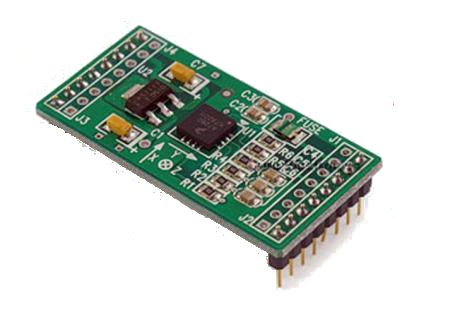
\includegraphics[height=5cm]{acelerometro}
	\caption{Módulo acelerómetro}
	\label{fig:modulo_acelerometro}
\end{figure}	

\subsection{Bluetooth}
\label{subsec:bluetooth}
Bluetooth é uma tecnologia padrão para comunicações sem fios à escala global, que liga dispositivos que se encontrem separados por curtas distâncias e encontra-se integrada em biliões de produtos no mercado atual, fazendo a ligação à Internet das Coisas (Internet of Things). Esta tecnologia utiliza pouca energia e cria uma pequena rede \emph{ad hoc} que emparelha dois a oito dispositivos remotamente através de um pequeno circuito que comunica utilizando ondas rádio, sendo possível conectar produtos como colunas de som, luzes, televisões, garrafas de água ou até brinquedos.
\begin{figure}[htbp]
	\centering
	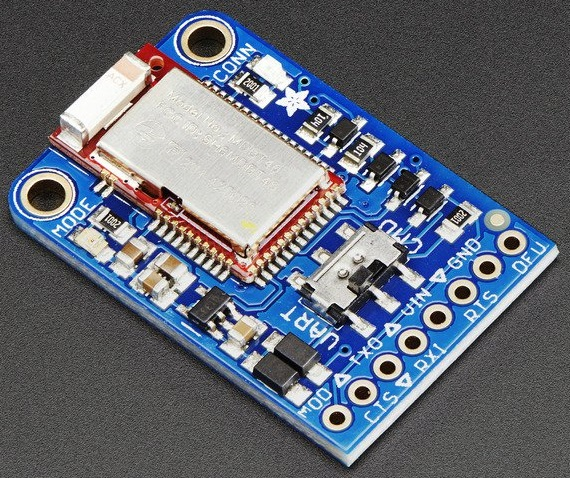
\includegraphics[height=5cm]{bluetooth}
	\caption{Módulo bluetooth}
	\label{fig:modulo_bluetooth}
\end{figure}

\subsection{Wi-fi}
\label{subsec:wi-fi}
Wi-fi, abreviatura de Wireless Fidelity (fidelidade sem fios) é uma tecnologia que utiliza ondas rádio para fornecer ligação a uma rede e é estabelecida utilizando adaptadores sem fios para criar ponto de acesso (\emph{hotspot}) que permite aos utilizadores obterem ligação ao serviço de Internet, desde que estejam ligados a ele. É necessário um adaptador sem fios para transmitir o sinal via rádio, que é enviado para um descodificador (router) através de uma antena, para que toda a informação possa ser enviada via Internet, utilizando várias frequências que permitem diversas velocidades de transmissão.
\begin{figure}[htbp]
	\centering
	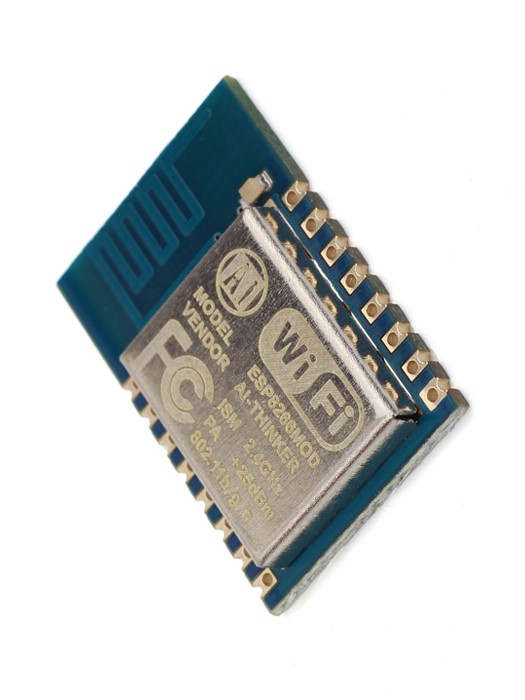
\includegraphics[height=5cm]{wi-fi}
	\caption{Módulo wi-fi}
	\label{fig:modulo_wifi}
\end{figure}

\subsection{GPS}
\label{subsec: gps}
GPS ou \emph{Global Positioning System} é um conjunto de 30 satélites igualmente espaçados que orbitam a Terra e fazem com que seja possível determinar a localização geográfica exata de um recetor que se encontre na superfície terrestre. A distribuição dos satélites no espaço está feita de modo a que em qualquer ponto do planeta seja possível contactar com quatro satélites. Cada um destes satélites contem um relógio atómico e um computador que em conjunto calculam a posição do recetor, incluindo a sua altitude, velocidade e direção (no caso de se estar a deslocar). O erro de precisão da posição do recetor é aproximadamente dez metros para a maior parte dos equipamentos atuais mas pode ser reduzida a um metro para equipamentos militares. O facto de ser bastante utilizado à escala mundial permite que tenha um custo bastante reduzido, sendo possível encontrar um destes recetores na maioria dos telemóveis fabricados no presente.
\begin{figure}[htbp]
	\centering
	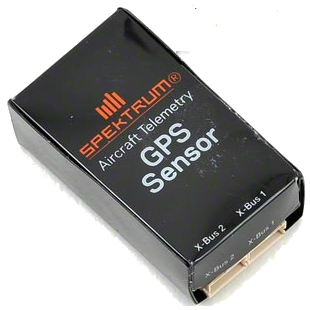
\includegraphics[height=5cm]{gps}
	\caption{Distribuição dos satélites GPS}
	\label{fig:distribuicao_dos_satelites_gps}
\end{figure}